\documentclass{article}
\usepackage[T1]{fontenc}
\usepackage[french]{babel}
\usepackage{amssymb}
\usepackage{fullpage}
\usepackage{graphicx}
%
% Environnement "exercice"
%
\newcounter{numexercice}
\newenvironment{exercice}{\addtocounter{numexercice}{1}\par\bigskip\noindent{\large \bf Exercice \thenumexercice\par}}{}
%
% Ensembles de nombres
%
\newcommand{\N}{\mbox{\rm I$\!$N}}
\newcommand{\Z}{\mbox{\rm \lower0.3pt\hbox{$\angle\!\!\!$}Z}}
\newcommand{\Q}{\mbox{\rm $~\vrule height6.5pt width0.5pt depth0.3pt\!\!$Q}}
\newcommand{\R}{\mbox{\rm I$\!$R}}
\newcommand{\C}{\mbox{\rm $~\vrule height6.5pt width0.5pt depth0.3pt\!\!$C}}
%
%%%%%%%%%%%%%%%%%%%%%%%%%%%%%%%%%%%%%%%%%%%%%%%%%%%%%%%%%%%%%%%%%%
%
\title{\textbf{TD MADIS : algorithme de Roy-Warshall}}
\begin{document}
\maketitle

Le problème, étant donné un graphe $G=(X,U)$ à $n$ sommets indicés de
1 à $n$, est de déterminer la fermeture réflexo-transitive de $G$ : le
graphe $\tau(G) = (X,\tau(U))$ ; rappelons que $(x,y)$ est un arc de
$\tau(G)$ si et seulement si $x=y$ ou bien s'il existe un chemin de
$x$ vers $y$ dans $G$. Soit $M$ la matrice d'adjacence binaire associée à $G$.
On rend $G$ réflexif par ajout d'une boucle en tout sommet n'en
comportant pas. On suppose désormais que $\forall i \in \{1,...,n\}
\mbox{, } m_{ii}=1$.

Considérons l'opérateur $\theta_r$ qui, appliqué à $G$, construit le
graphe $\theta_r(G)$ : par définition $\theta_r(G)$ comporte les arcs
de $U$ ainsi que tout arc $(i,j)$ tel qu'existent dans $U$ les arcs
$(i,r)$ et $(r,j)$. Autrement dit, $\theta_r$ enrichit $G$ des arcs
$(i,j)$ (si ceux-ci n'existaient pas) tels qu'il existe un chemin de
longueur deux de $i$ vers $j$ passant par $r$.

L'algorithme de Roy-Warshall consiste alors à :
\begin{itemize}
\item appliquer $\theta_1$ à $G$
\item appliquer $\theta_2$ à $\theta_1(G)$
\item appliquer $\theta_3$ à $\theta_2(\theta_1(G))$
\item ...
\item et enfin à appliquer $\theta_n$ à $\theta_{n-1}(...\theta_2(\theta_1(G)))$
\end{itemize}


\textbf{1. }Appliquer cet algorithme au graphe $G$ de la figure~\ref{fig:graphe},
après avoir établi $M$. Exprimer les composantes fortement connexes de
$G$.

\begin{figure}[htbp]
  \begin{center}
    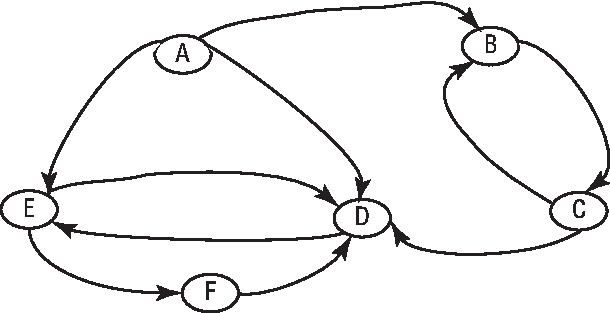
\includegraphics[width=6cm]{td_rw_pdf.pdf}
    \caption{Graphe $G$}
    \label{fig:graphe}
  \end{center}
\end{figure}
\textbf{2. } Preuve de l'algorithme

\textbf{2.1 } Soit $M^{(r)}$ la matrice booléenne associée à
$\theta_r(G)$. Montrer que
\begin{equation}
  m_{ij}^{(r)} = m_{ij} \dotplus m_{ir}m_{rj}
\end{equation}

\textbf{2.2} Montrer que les opérateurs $\theta_r$ et $\theta_s$
 ($1 \leq r,s \leq n$) commutent.

\textbf{2.3} Montrer que l'opérateur $\theta_r$ est idempotent.

\textbf{2.4} Montrer que la composition des opérateurs $\theta_{.}$
est associative.

\textbf{2.5} Montrer que $\theta = \theta_1 \circ  \theta_2 \circ
... \circ \theta_n$ a au moins pour effet d'ajouter à $G$ les arcs
$(i,j)$ n'existant pas dans $U$ tels qu'il existe un chemin de
longueur 2 de $i$ vers $j$ dans $G$ ; que peut-on en déduire pour
$\theta^2 = \theta \circ \theta$ ?

Prouver alors que $\theta^{n-2}(G) = \tau(G)$.

\textbf{2.6 } En déduire que $\theta(G) = \tau (G)$.

\textbf{3. } Evaluer la complexité de cet algorithme.
\end{document}
